
Non-resonant standard model $WW$ production is a major background to
VBF \hww: \textapprox{19\%} in the \emme SR and \textapprox{9\%} in
the \eemm SR. SM \wwtwoj processes are split into two
categories. Processes in which the partons producing the two jets
arise from QCD vertices are labeled ``QCD \ww''. Two examples of LO QCD \ww
diagrams are shown in
Figures~\ref{chap:analysis:fig:qcd_ww_tchan}\subref{chap:analysis:fig:qcd_ww_schan}. In
both examples, the outgoing partons are correlated by color exchange,
making them more central in rapidity and resulting in more soft QCD
activity between the two. The second category, ``EW \ww'', refers
to processes in which the two jets are produced via electroweak
vertices. An example of such a process is one in which the two
incoming quarks radiate virtual gauge bosons that then interact via
two triple gauge couplings to produce a pair of $W$s, shown in
figure~\ref{chap:analysis:fig:ew_ww_tchan}. Another example of such a
process, shown in figure~\ref{chap:analysis:fig:ew_ww_qgc}, is when the
two radiated virtual bosons produce a pair of $W$s through a quartic
gauge coupling. By definition, EW \ww~processes do no have any QCD
vertices at tree level, and as a result, the total EW \ww rate is
significantly smaller than that of QCD \ww. However, because EW \ww
and VBF \hww have similar color structure resulting in a large rapidity
gap between the final state jets, the EW \ww prediction in the most
sensitive BDT bins is non-negligible. In fact, QCD and EW \ww contribute about the same
number of events in the high BDT bin, \textapprox{0.25} events. 

\begin{figure}[h]
    \centering
    \subfigure[]{
    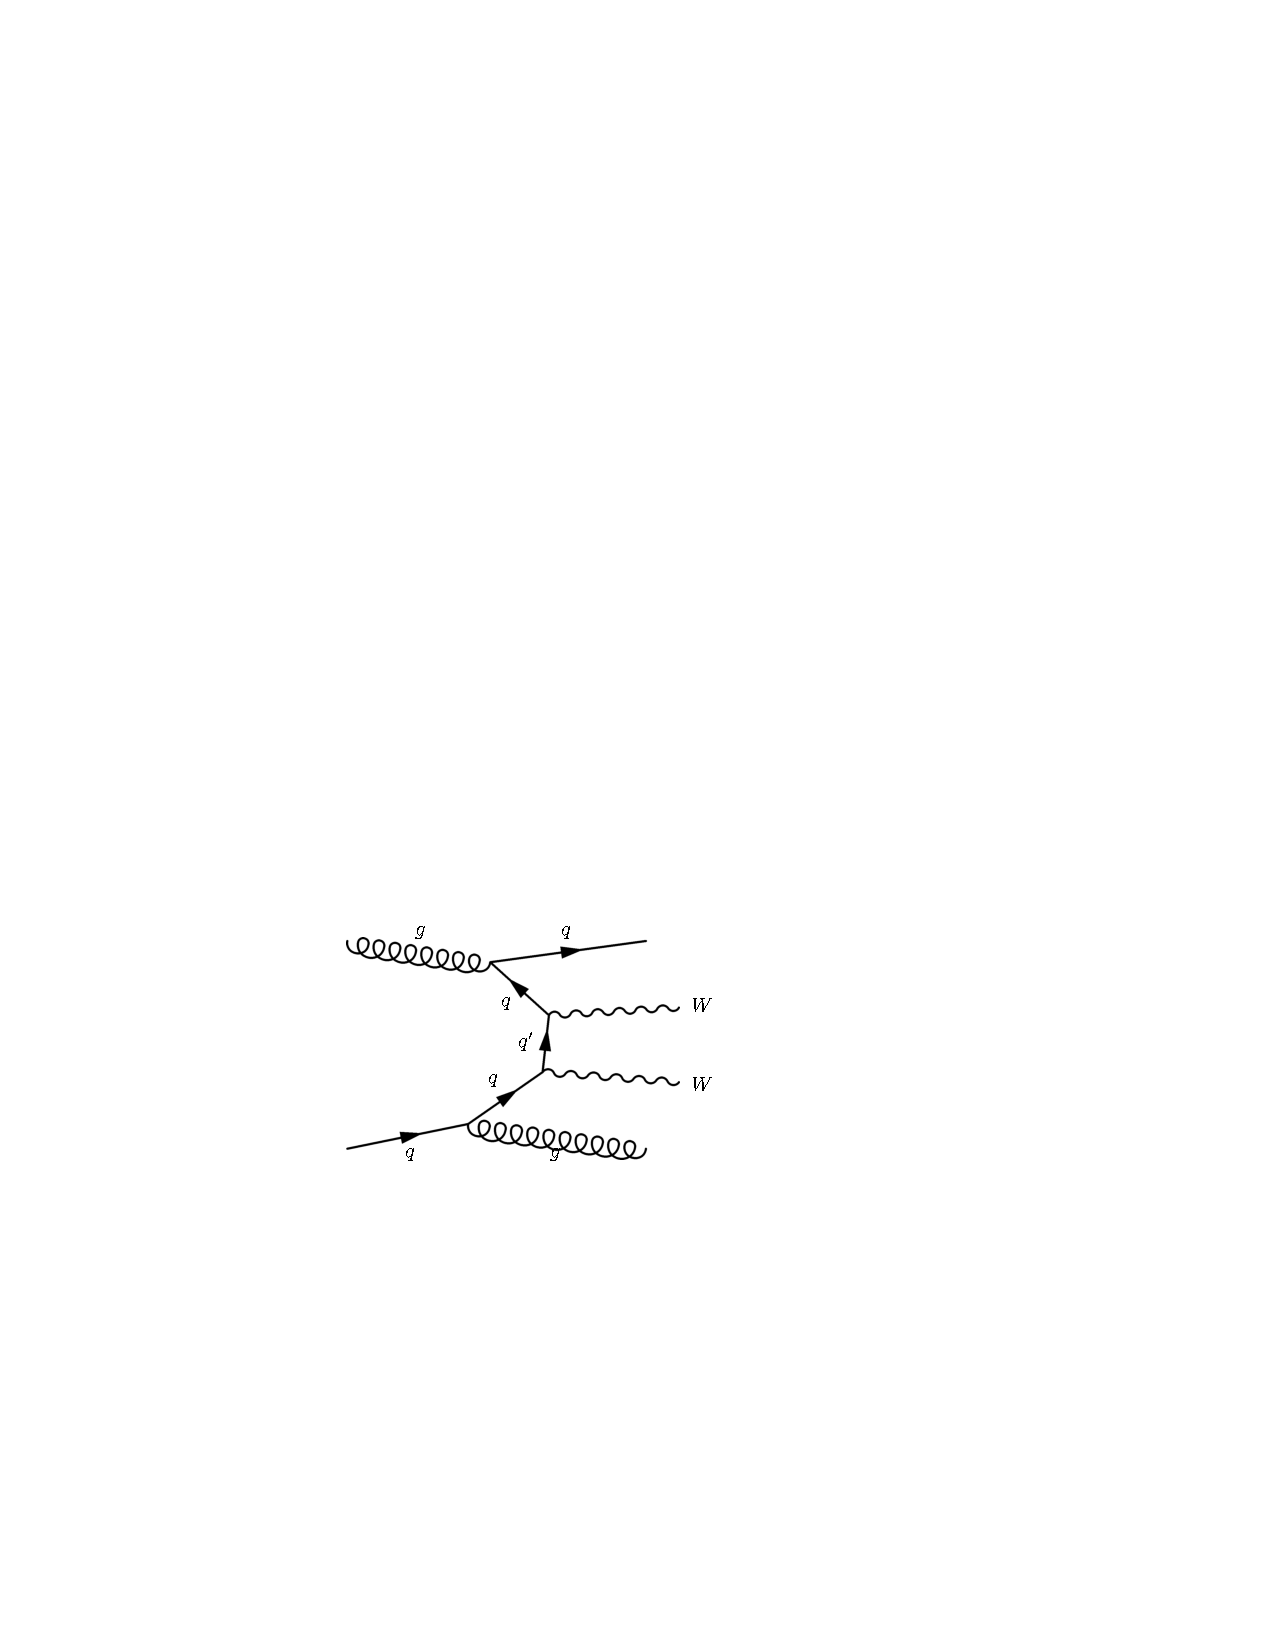
\includegraphics[width=0.4\textwidth]{analysis/ww/qcd_ww_tchan.pdf}
    \label{chap:analysis:fig:qcd_ww_tchan}
    }
    \subfigure[]{
    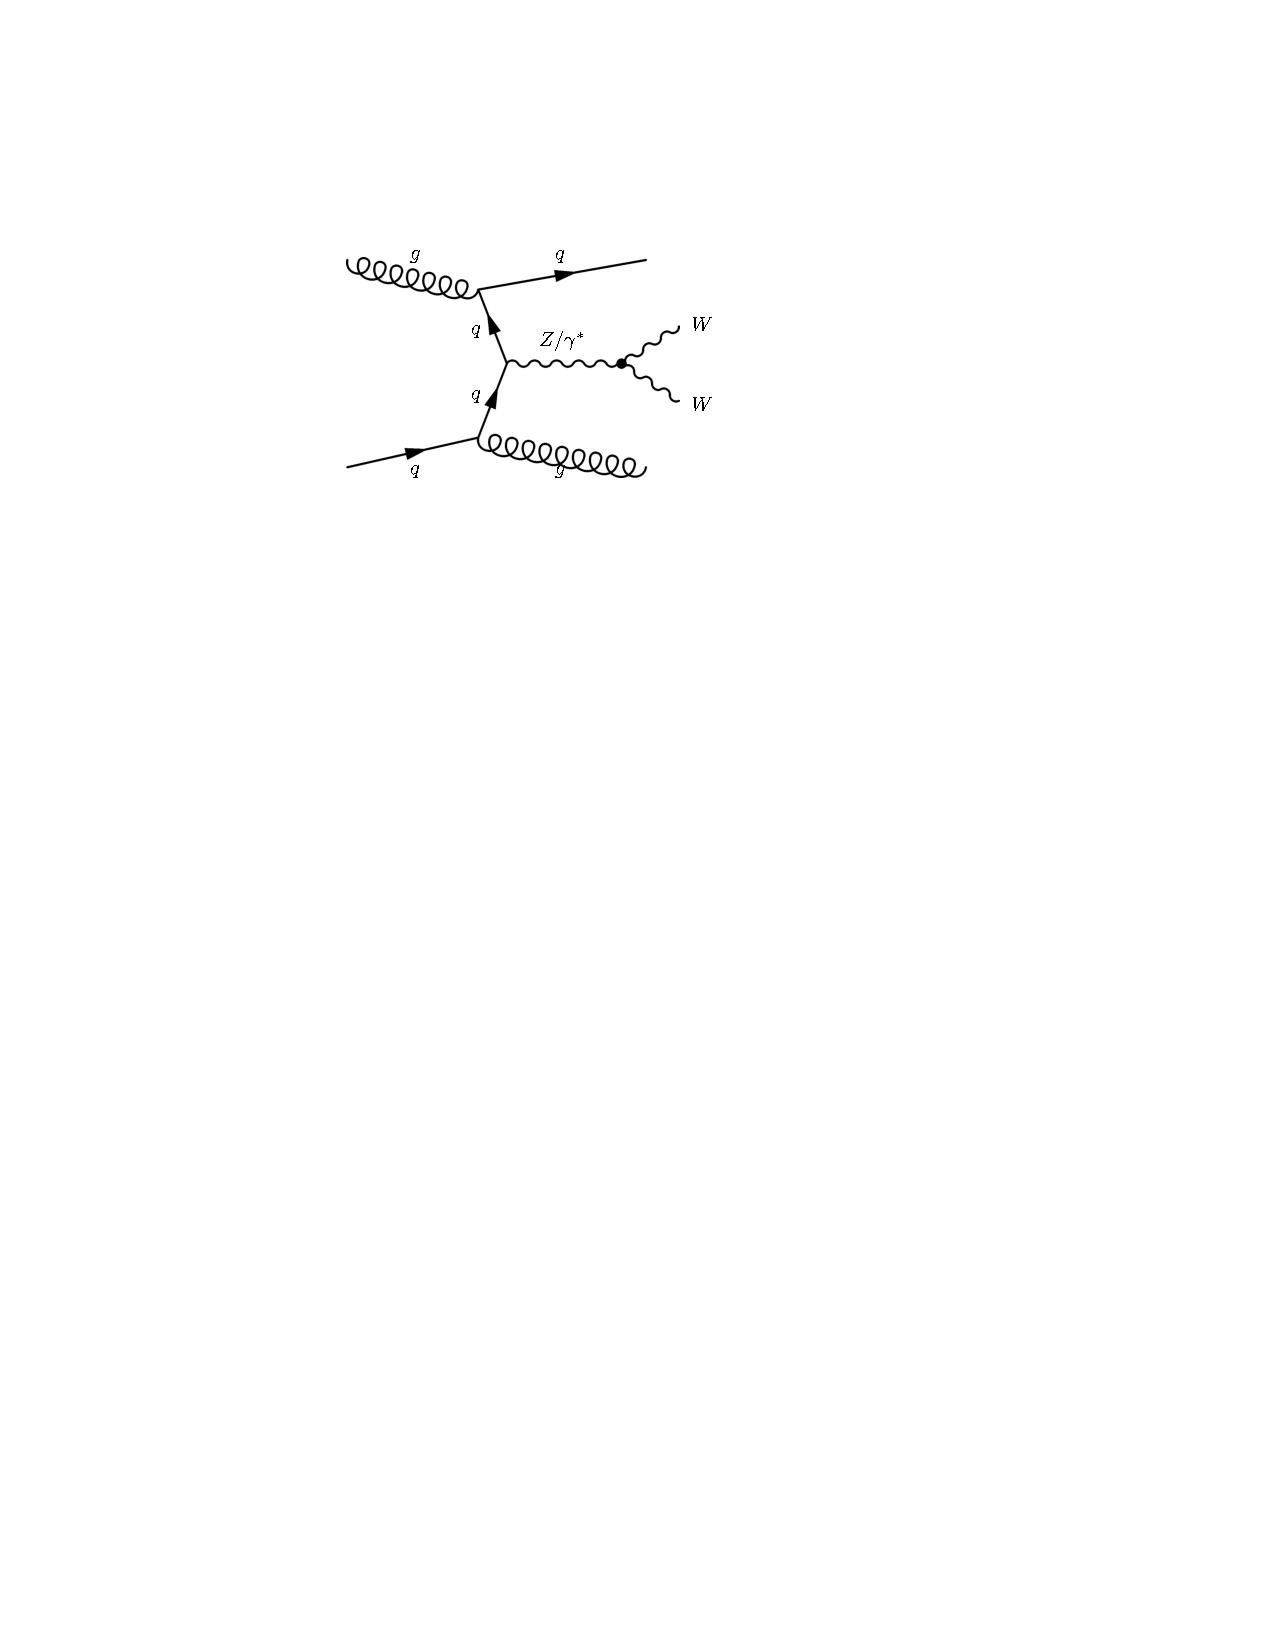
\includegraphics[width=0.4\textwidth]{analysis/ww/qcd_ww_schan.pdf}
    \label{chap:analysis:fig:qcd_ww_schan}
    }
    \subfigure[]{
    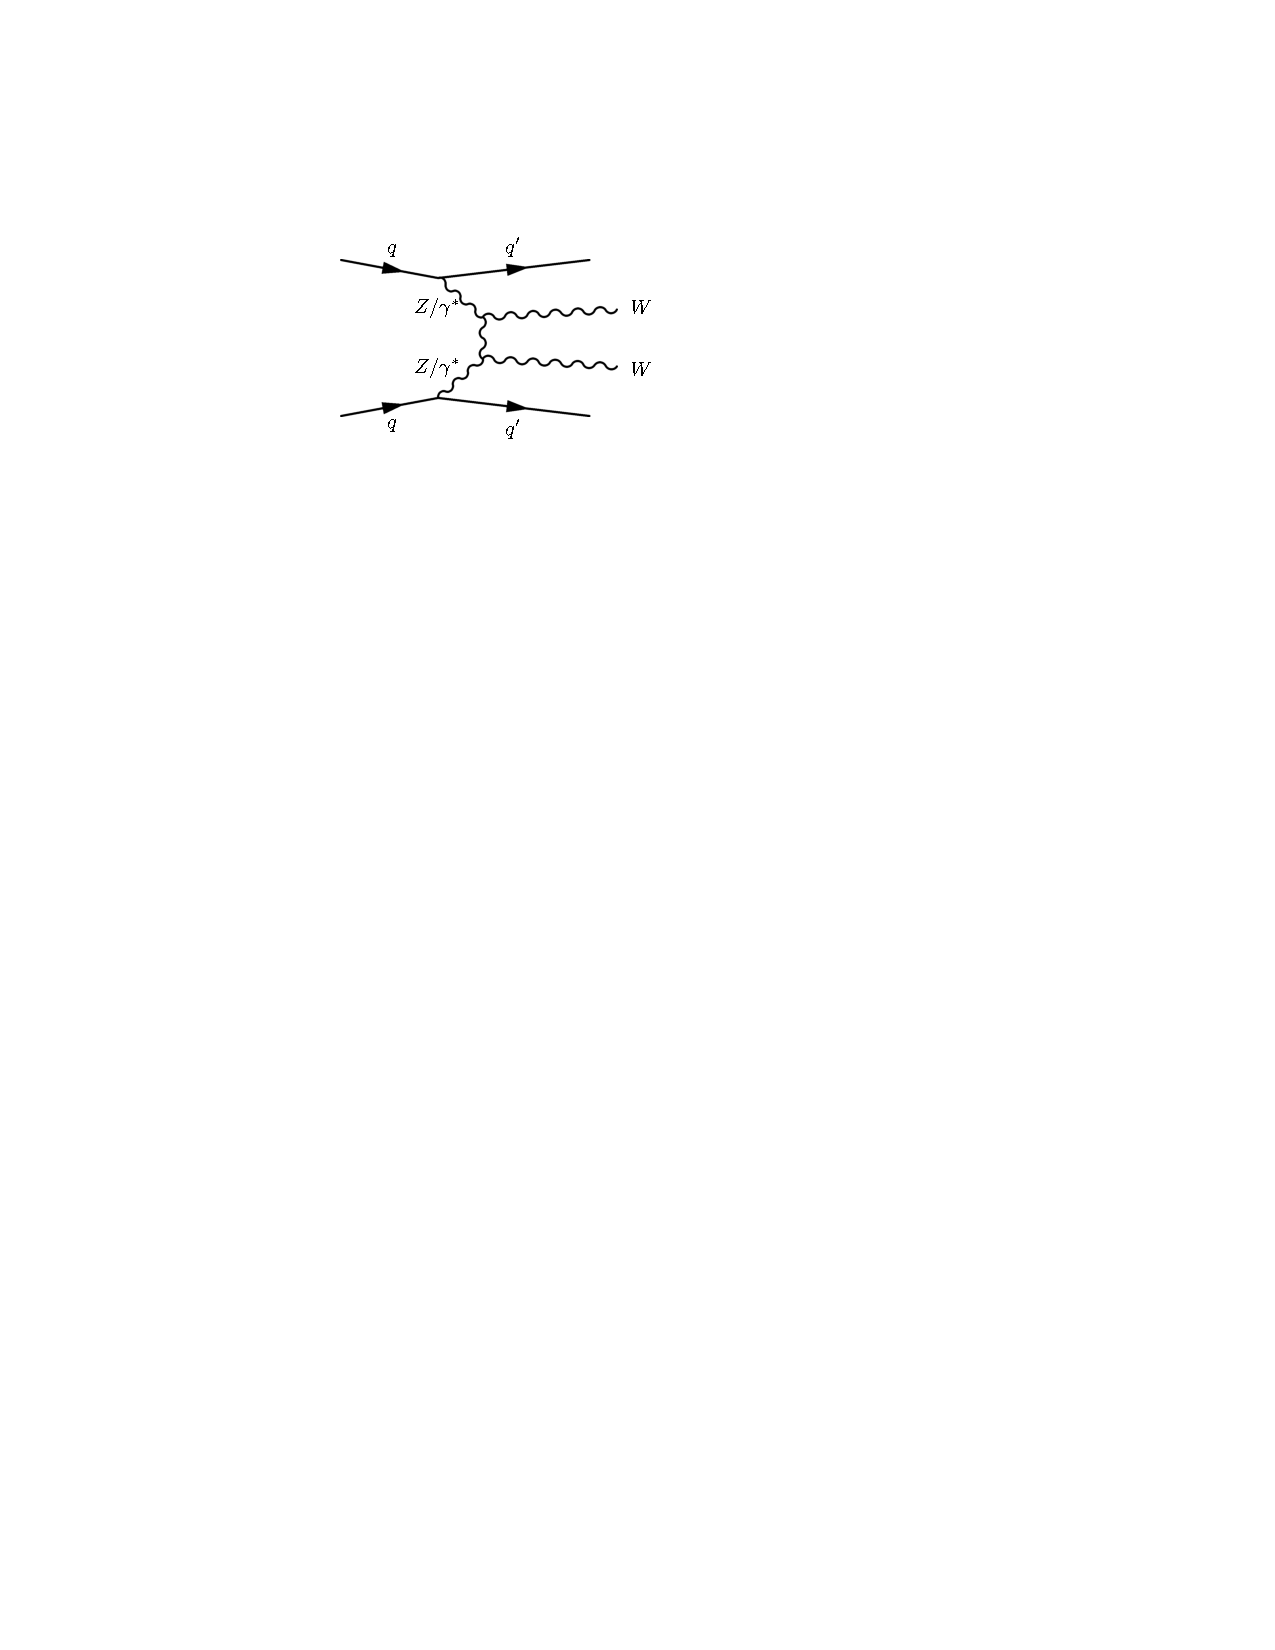
\includegraphics[width=0.4\textwidth]{analysis/ww/ew_ww_tchan.pdf}
    \label{chap:analysis:fig:ew_ww_tchan}
    }
    \subfigure[]{
    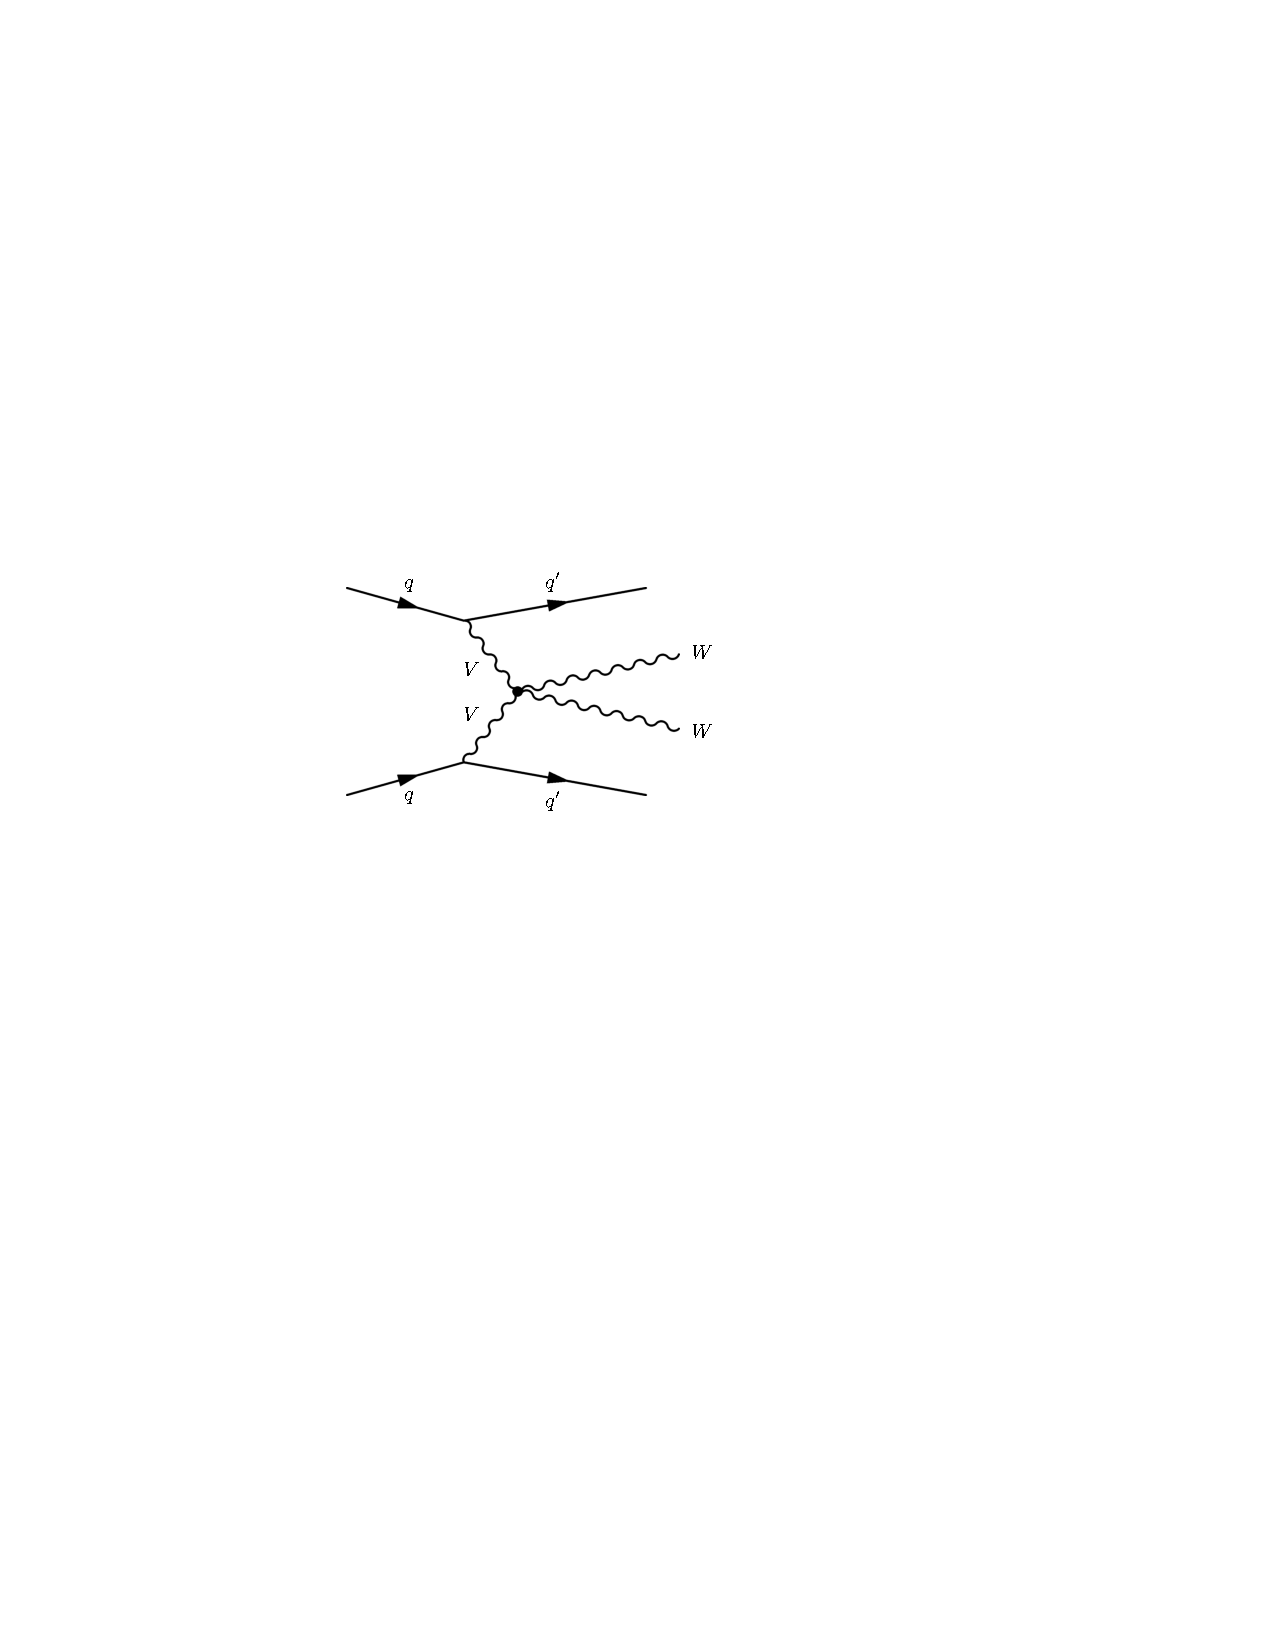
\includegraphics[width=0.4\textwidth]{analysis/ww/ew_ww_qgc.pdf}
    \label{chap:analysis:fig:ew_ww_qgc}
    }
    \caption[LO Feynman diagrams for SM \ww.]{LO Feynman diagrams for
    SM \ww.~\subref{chap:analysis:fig:qcd_ww_tchan}
    and~\subref{chap:analysis:fig:qcd_ww_schan} are examples of
    QCD \ww processes, and~\subref{chap:analysis:fig:ew_ww_tchan}
    and~\subref{chap:analysis:fig:ew_ww_qgc} are EW \ww processes.}
\label{chap:analysis:fig:ww_feyn_diag}
\end{figure}

The QCD \ww prediction is from \SHERPA 1.4.1, which is used to simulate the
hard-scatter, parton shower, and hadronization for all
$q\bar{q}/qg/\bar{q}g\rightarrow{WW}$ diagrams. Events are generated
at LO in QCD with up to three jets at matrix element level, and the $W$ bosons are
forced to decay leptonically. The overall normalization is
scaled to the total \ww cross section at \sqrts$=8$~\tev, as computed
in \MCFM: $\sigma_{tot}(\wwlnln) = 5.679$~pb. Given that the branching
fraction of $W\rightarrow{\ell\nu}$ is 0.1082 and there are nine
lepton combinations, the corresponding total cross section is
$\sigma_{tot}(\ww) = 53.90$~pb. The total \ww cross section has been
measured in ATLAS in the \ww leptonic decay channels and the exclusive zero jet
bin~\cite{bib:ww_cross_section}. The result, which includes resonant \ww production from $H$, is
$\sigma_{tot}(WW) = 71.4^{+1.2}_{-1.2} \textrm{(stat)} ^{+5.0}_{-4.4}
\textrm{(syst)}^{+2.2}_{-2.1}\textrm{(lumi)}$~pb, significantly larger
than the \MCFM computation which includes $H$, $\sigma_{MCFM}(WW) =
58.7^{+3.0}_{-2.7}$~pb. However, the ATLAS measurement is done in a phase space
region that is orthogonal to this analysis, and in fact, the \MCFM
calculation does not include diagrams with two partons in the final
state. The normalization in the 2j bin relies on the LO jet multiplicity prediction
from \SHERPA. 

To assess the uncertainty, \MADGRAPH interfaced
with \PYTHIA 6 for showering is used. The sample which is generated is
also inclusive, with up to three partons generated at the matrix element
level. These final state partons are then showered in \PYTHIA with the
MLM matching scheme (reference) at a scale of 20~\gev. The PDF in
both \MADGRAPH and \PYTHIA is \cteqsixl, and the underlying event tune
is AUET2B (reference). A modeling uncertainty is computed by comparing
the truth level predictions from \SHERPA and \MADGRAPH. As described
in section~\ref{chap:analysis:section:top}, the BDT inputs are
evaluated at truth level, and the resulting distortion of the BDT
spectrum is taken as an uncertainty. For the comparison, the two
samples are scaled to the integrated luminosity with their respective
cross sections. The \MADGRAPH cross section computed after showering is
4.55~pb compared to the \SHERPA cross section of 5.679~pb. This
approach folds together both kinematic and normalization differences
between the two generators. Displayed in
figure~\ref{chap:analysis:fig:qcdww_gen_uncert} is the truth level BDT
response. In light of the differences, uncertainties of 14\%, 8\%, and
12\% are assigned. 

\begin{figure}[h]
    \centering
    \subfigure[QCD \ww]{
    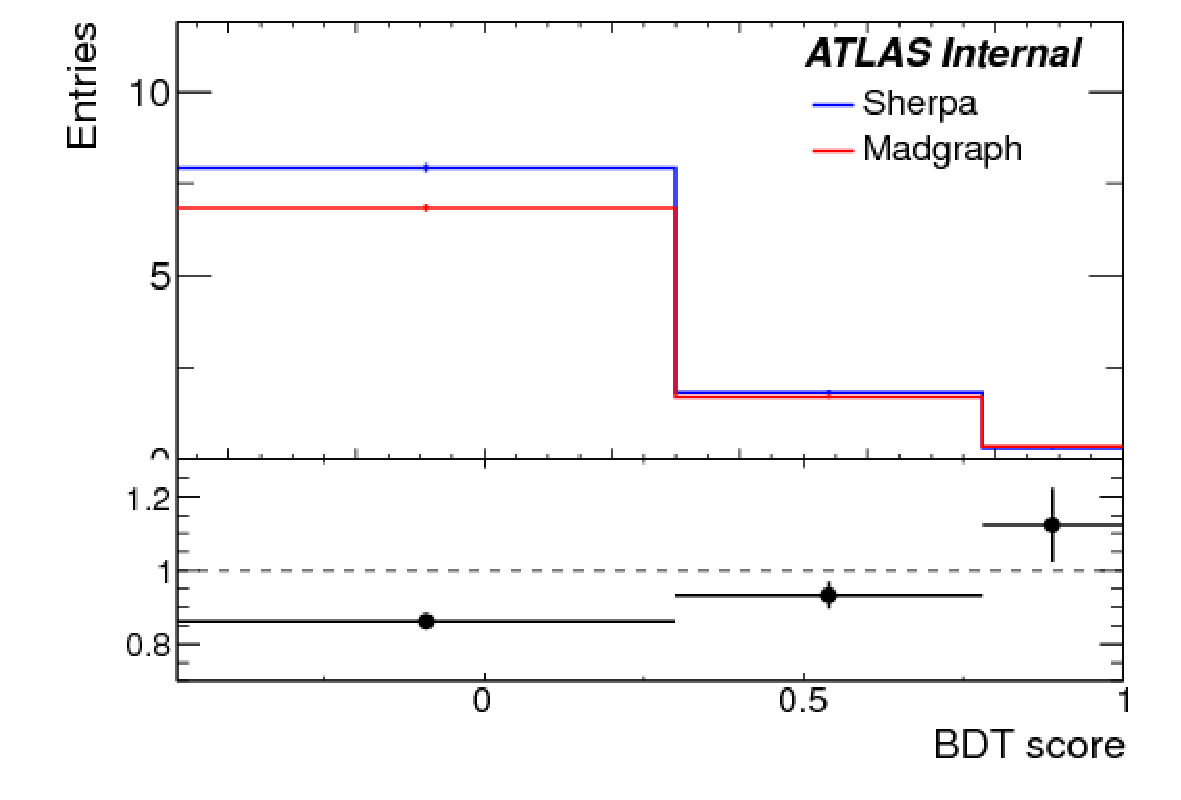
\includegraphics[width=0.45\textwidth]{analysis/ww/ww_shape_sys_qcd.pdf}
    \label{chap:analysis:fig:qcdww_gen_uncert}
    }
    \subfigure[EW \ww]{
    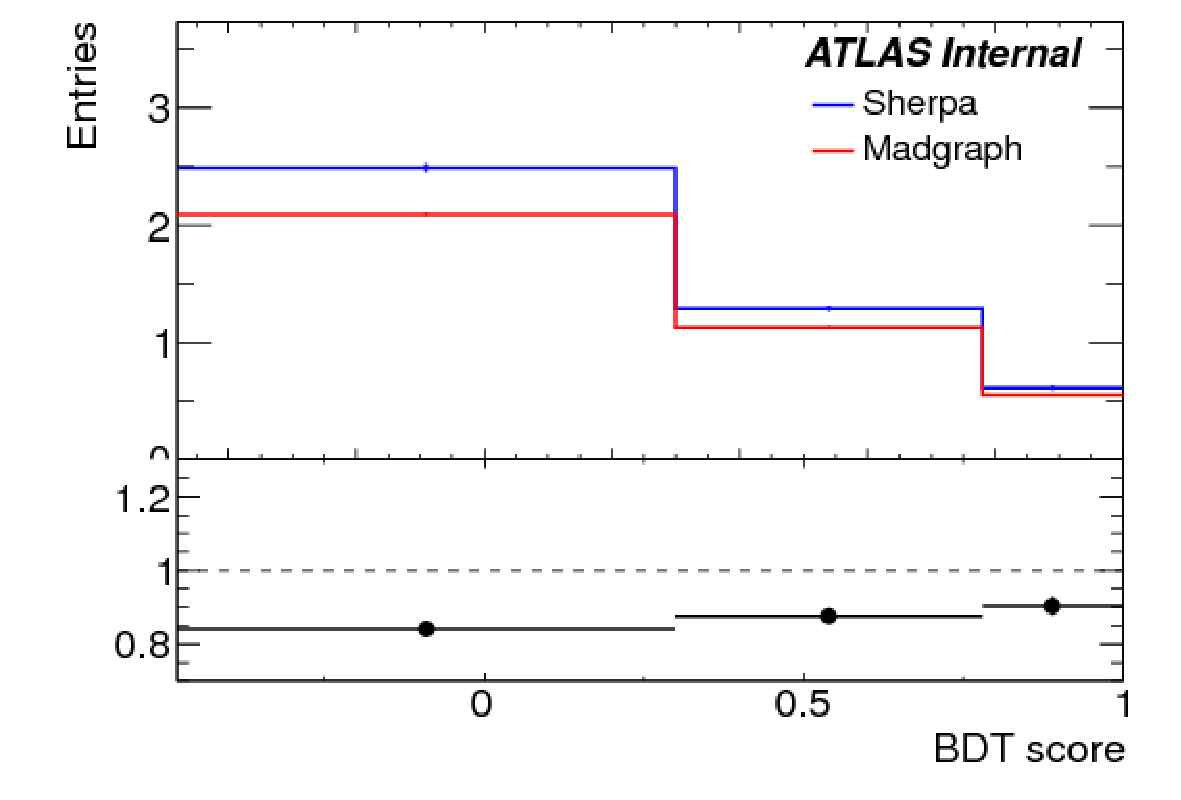
\includegraphics[width=0.45\textwidth]{analysis/ww/ww_shape_sys_ew.pdf}
    \label{chap:analysis:fig:ewww_gen_uncert}
    }
    \caption[Comparison of \MADGRAPH and \SHERPA predictions
    for \ww.]{Comparison of \MADGRAPH and \SHERPA predictions for \ww.}
\label{chap:analysis:fig:ww_gen_uncert}
\end{figure}

In addition to a generator modelling uncertainty, the uncertainty from
the choice of QCD scale in the matrix element calculation is
assessed. The factorization and renormalization scales in \MADGRAPH,
which are varied dynamically event-by-event, are coherently scaled up and down by
a factor of two. After showering in \PYTHIA, the samples are scaled to
integrated luminosity and the event yield prediction in the
truth-level SR is evaluated. With $\mu_R=\mu_F=\mu_{\textrm{default}}/2$, the
predicted number of events in the SR is $27\%$ higher than the default
scale choice, while with $\mu_R=\mu_F=2\mu_{\textrm{default}}$, the prediction
falls by $2.6\%$. The larger of the two, $27\%$, is assigned as the
uncertainty. This uncertainty is consistent with the LO $\sigma(WW)$ uncertainty
computed at \sqrts$=7$~\tev ~\cite{bib:Melia:2011dw}, though in a
looser phase space region. Additional QCD \ww uncertainties are
summarized in table~\ref{chap:analysis:tab:ww_theory_uncerts}.

\begin{table}
\begin{center}
\renewcommand{\arraystretch}{1.2}
%\resizebox{0.8\textwidth}{!}{
    \begin{tabular}{| l | c | c |}
    \hline
    Source & QCD \ww & EW \ww \\
    \hline \hline
    Generator modeling & (12\%,8\%,12\%) & (16\%,12\%,10\%) \\
    QCD scale & 27\% & 10\% \\
    PDF ($\sigma$) & 4\% & 3\% \\
    PDF (acceptance) & 2\% & $-$ \\
    QCD-EW interference & $-$ & 2\% \\
    Higgs interference & $-$ & 1.2\% \\
    \hline
    \end{tabular}
%}
\caption[Summary of \ww~theory uncertainties.]{Summary of \ww~theory uncertainties.}
\label{chap:analysis:tab:ww_theory_uncerts}
\end{center}
\end{table}

For EW \ww, a generator modeling uncertainty is computed by comparing the
prediction of \SHERPA to that of \MADGRAPH interfaced
with \PYTHIA. The cross section computed in \MADGRAPH is 27.37~fb,
30\% lower than that of \SHERPA, resulting in fewer events
predicted. A comparison of the absolute predictions for the two
generators is shown in
figure~\ref{chap:analysis:fig:ewww_gen_uncert}, corresponding to
uncertainties of 16\%, 12\%, and 10\% in BDT bins. 

The QCD scale uncertainty is computed at LO
in~\cite{bib:Jager:2006zc}. The uncertainty is computed in a generic
VBF phase space region with cuts on \dyjj and \mjj. Such a region is
expected to significantly overlap with the SR defined by the BDT. The
resulting uncertainty, computed by varying $\mu_F$ and extracting the
cross section, is 10\%. 

Remaining theory uncertainties for EW \ww are shown in
table~\ref{chap:analysis:tab:ww_theory_uncerts}. The uncertainty from interference
between EW \ww and Higgs-mediated \ww is computed by comparing the
cross section of \ww and \hww diagrams without interference to the
corresponding cross section with interference. At a Higgs mass
hypothesis of $m_H = 125$~\gev, the uncertainty is 1.2\%, while at
$m_H = 150$~\gev, the uncertainty is 6.4\%. Because these are small
with respect to the modeling and QCD scale uncertainties, they are
neglected in the fit. An uncertainty due to interference between QCD
and EW \ww processes is evaluated in a similar way and found to
be \textapprox{2\%}. This, too, is neglected in the fit. 




